\subsubsection{Présentation du récepteur}
La Figure \ref{fig:filtre1} illsutre le nouveau récepteur que nous allons implémenter dans un premier temps.

Pour l'instant nous supposons que les phases des cosinus du signal initial, avant transport, et celles du signal après transport, au niveau du récepteur sont les mêmes.
Détaillons les calculs de ce récepteur :\\
Soit :
\[
   \left\{
   \begin{array}{rcl}
      I_{0, 0} & = & \int_{0}^{T_s}  cos( 2 \pi F_0 t + \phi_0 )(cos(2\pi F_0t+\phi_0) dt \\
      I_{0, 1} & = & \int_{0}^{T_s}  cos( 2 \pi F_0 t + \phi_0 )(cos(2\pi F_0t+\phi_1) dt \\
      I_{1, 0} & = & \int_{0}^{T_s}  cos( 2 \pi F_0 t + \phi_1 )(cos(2\pi F_0t+\phi_0) dt \\
      I_{1, 1} & = & \int_{0}^{T_s}  cos( 2 \pi F_0 t + \phi_1 )(cos(2\pi F_0t+\phi_1) dt \\
   \end{array}
   \right.
\]
De plus, on rappelle :

\[
   \begin{array}{rcl}
      x(t) & = & (1-NRZ(t)) \times cos(2\pi F_{0}t+\phi_{0}) + NRZ(t)\times cos(2\pi F_{1}t+\phi_{1}) \\
   \end{array}
\]
A l'étape \textcolor{Red}{2.1} (Figure \ref{fig:filtre1}) on multiplie $x(t)$ par $cos(2\pi F_0t)$. De même, à l'étape \textcolor{Red}{32.2}, on multiplie $x(t)$ par $cos(2\pi F_1t)$. Puis, aux étapes
\textcolor{Red}{3.1} et \textcolor{Red}{3.2}, on calcule les intégrales des résultats des étapes précédentes. Enfin, à l'étape \textcolor{Red}{4}, on soustrait l'un à l'autre.
Au final on trouve :
\begin{dinglist}{111}
   \item Si $NRZ = 0$ :
   \[
      \begin{array}{rclcl}
         R & = & I_{0, 1} - I_{0, 0} & \approx & -\frac{T_s}{2} < 0
      \end{array}
   \]
   \item Si $NRZ = 1$ :
   \[
      \begin{array}{rclcl}
         R & = & I_{1, 1} - I_{1, 0} & \approx & \frac{T_s}{2} > 0
      \end{array}
   \]
\end{dinglist}
Ainsi, si la sortie du récepteur est positive, le bit retrouvé est 1, sinon, le bit retrouvé est 0.

\begin{figure}[H]
   \centering
   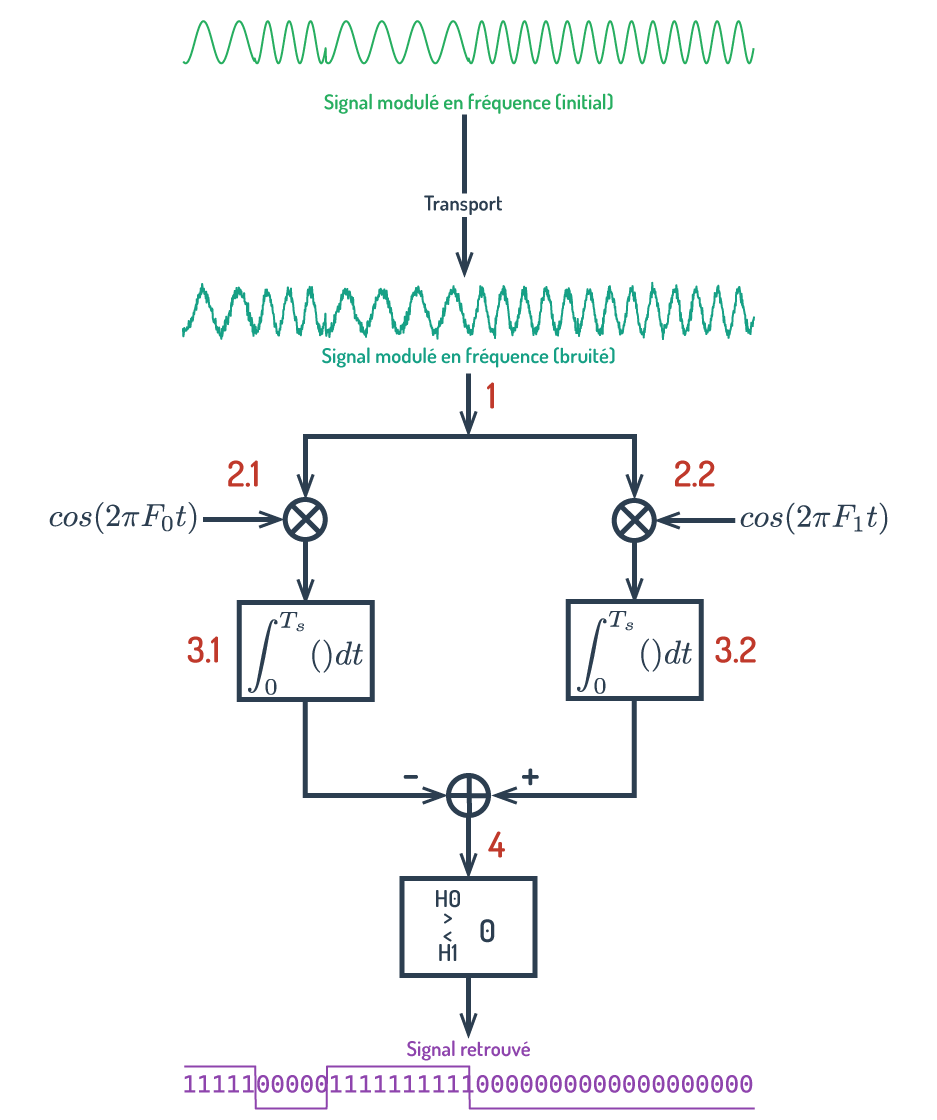
\includegraphics[scale=0.4]{partie-3/sous-partie-1/filtre1.png}
   \caption{Schéma de démodulation FSK avec synchronisation idéale} \label{fig:filtre1}
\end{figure}
\subsubsection{Implémentation du récepteur}
\begin{lstlisting}[caption=Récepteur V21 à synchronisation idéale, label=code:syn-ideal]
x0 = x .* cos(2 * pi * F0 * t + phi0);
x1 = x .* cos(2 * pi * F1 * t + phi1);

x0_reshape = reshape(x0, Ns, Nb_bit);
X0 = sum(x0_reshape * Ts, 1);

x1_reshape = reshape(x1, Ns, Nb_bit);
X1 = sum(x1_reshape * Ts, 1);

X2 = X1 - X0;
Donnee_retrouve_2 = X2 > 0;

Nb_erreur_2 = sum(Donnee ~= Donnee_retrouve_2);
taux_erreur_2 = Nb_erreur_2 / Nb_bit
\end{lstlisting}

Le \lstinline{phi0} et \lstinline{phi1} des lignes 1 et 2 sont les mêmes que ceux déifnis aux lignes 2 et 3 du Code \ref{code4}.
Toujours pour un rapport signal sur bruit de 50dB, on trouve on taux d'erreur de 0\%.